\begin{minipage}[t]{170mm}
\vspace{3mm}
\begin{center}
\section*{Befriet af dværge!}
\end{center}

\emph{Hej-Ho}

Her er Erebor, DBC sender til MatCamp 

\emph{Hej-Ho}

I hører os i stridsøksebåndet. 

Vi begynder med krigsnyhederne for Campen, herefter Dværgerådets proklamationer, de udencampske nyheder i øvrigt, en skildring af forholdene på Campen og en beretning om feernes sammenbrud på GDC.

Der foreligger endnu ikke nogen officiel meddelelse fra dværgenes side, om hvor langt Gimlis styrker er nået op i Vandrehallen. Campens presseansvarlige i fysiktårnet havde kl. 7 direkte kontakt med MatLab og på dette tidspunkt havde Gimlis tropper endnu ikke passeret døren til trappeopgangen. Det meddeles, at de små styrker tidligt i nat startede deres fremrykning fra fysikbadene på vej mod Campens undervisningslokaler. En øksekolonne nåede i nat døren med kortlæseren ved grænsen mellem fysik og matematik, kun fire meter fra vandrehallen. I de senest indløbne dværgefrontberetninger, hedder det sig, at situationen er så forvirrende, at der ikke er nogen officiel nyhed om, hvor langt dværgene er nået. Campens presseansvarlige meddeler videre i sit telegram kl. 7: Store deltagermængder samler sig i vandrehallen, alle laboratorietimer er aflyst, alle sociale møder udsat, og hele deltagerskaren venter utålmodigt på at give Gimlis øksebærere en hjertelig velkomst.

Der er på Campen en tiltagende følelse af, at der forhandles mellem dværgenes armé og Tandfeen \& Den Gode Fe, og at der vil blive indgået en aftale om overgivelse. Denne formodning støttes af den kendsgerning at feerne har erklæret kemi og biologi for åbne institutter. Det synes ikke fornuftigt for feerne frivilligt at opgive den temmelig stærke forsvarslinje ved kemi for så derefter at kæmpe på matematik.

Der er stor nervøsitet blandt feernes tropper. Nogle steder ser det ud som om de er ved at forberede sig til kamp. For eksempel har de bemandet befæstningerne ved sodavandsautomaterne foran MatLab, men adskillige andre steder er feerne øjensynligt utålmodige efter at komme til at overgive sig. 

Fysisk sekretariat har videregivet forlydender om, at hobbitternes kaffebryggere skulle være landet på matematisk bibliotek, og i dag gik der rygter på Campen om, at hobbitter har sneget sig ned ad trappen. Alle disse rygter savner ethvert belæg.

I nat blev der kæmpet voldsomt i MatLabs hyggehjørne, rundt om spilbordet, og der hørtes endog fingerknips. På matematisk bibliotek og på læsepladserne på anden sal havde fetropper været i indbyrdes regulær kamp.

\emph{Længere pause}

I dette øjeblik meddeles det, at Gimli har oplyst, at feernes tropper i D- og E-bygningen og på MatCamp har overgivet sig. Her er Erebor. Vi gentager: Gimli har i dette øjeblik meddelt, at feernes tropper i D- og E-bygningen og på MatCamp har overgivet sig.

\emph{Pause}

Vi fortsætter nu udsendelsen med at oplæse de to proklamationer, som Campens frihedsråd udsendte i nat, altså inden den meddelelse vi netop har givet:

'Hvad enten det kommer til kamp eller kapitulation, vil befrielseskampens sidste timer kræve endnu større disciplin og selvbeherskelse end hidtil. Ingen gruppe må gå til handling, før ordren er givet. Algebraikere, analytikere, vi stoler på jer.'

Feerne kom altså til fornuft og valgte kapitulationen. Det var en af de muligheder, Campens frihedsråd havde forudset i den proklamation, som vi netop har hørt, og som blev forfattet i nat. Nu, for nogle få minutter siden, erfarede vi fra Gimlis hovedkvarter, at fjenden i D- og E-bygningen og på Campen har kapituleret.

\emph{Den kanoniske matematikersang og Jeg er en matematiker fra HCØ afspilles}

\begin{center}
\vspace{3mm}
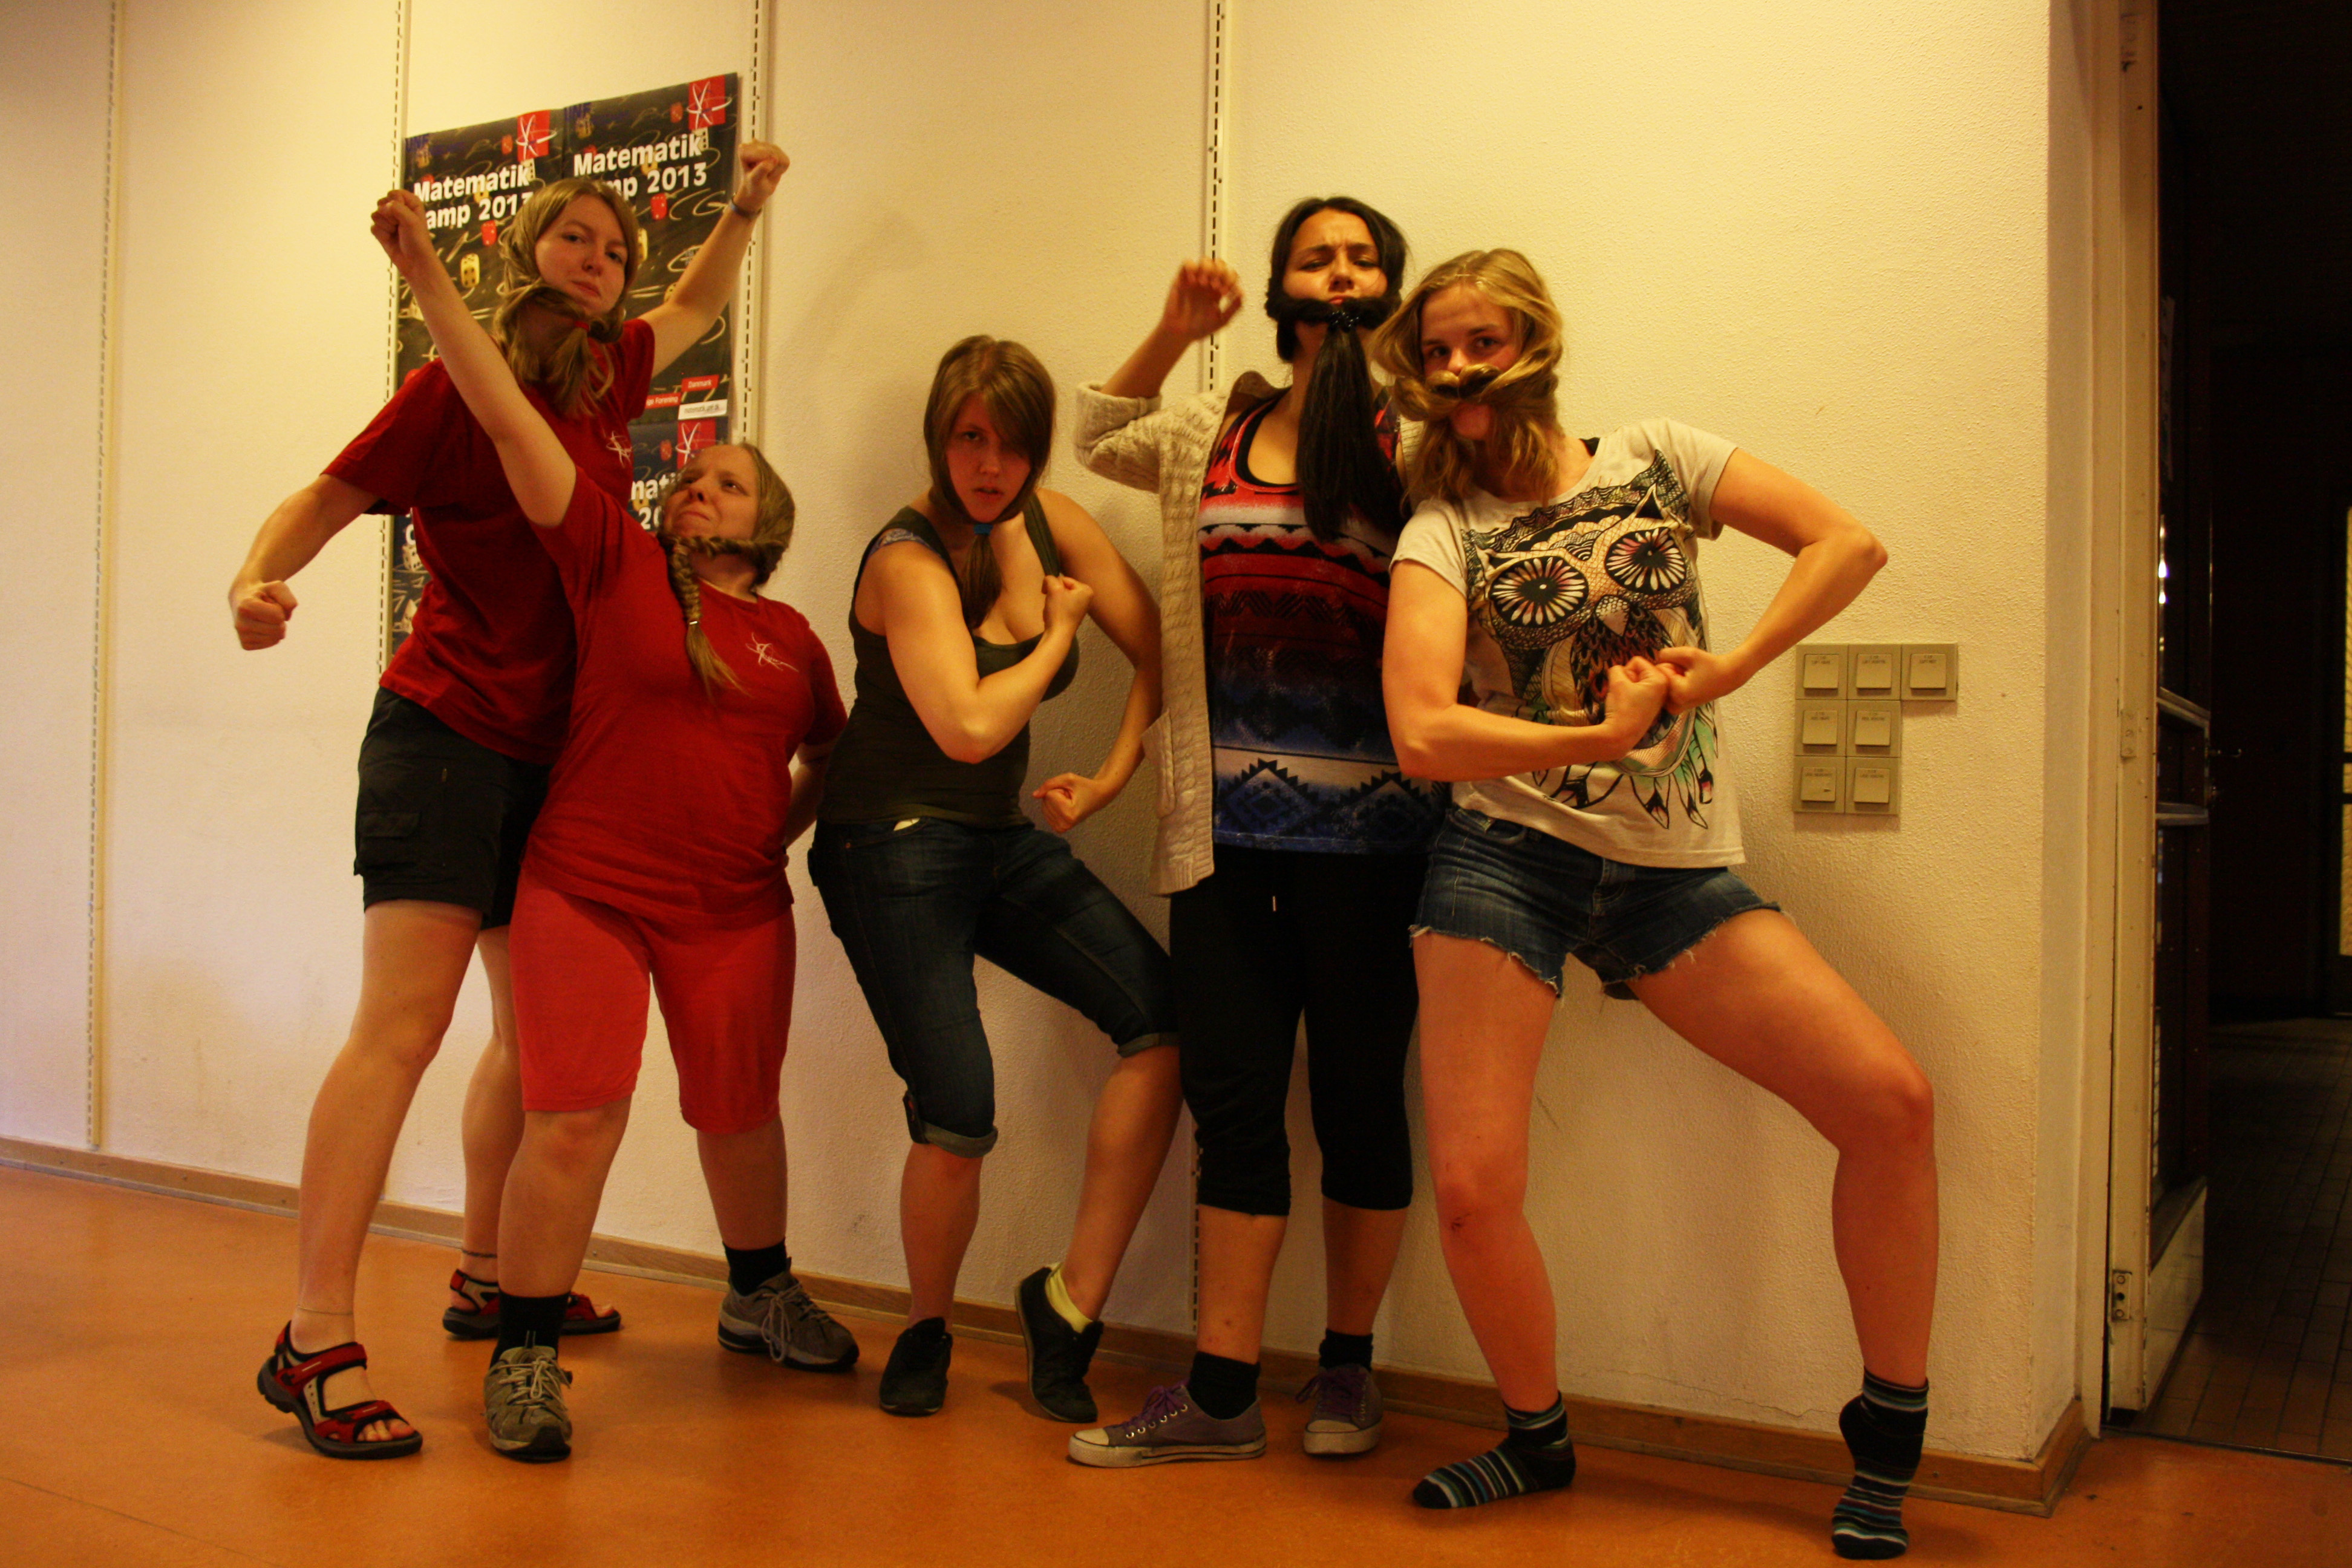
\includegraphics[width=130mm]{dvaergetropper.jpg}
\end{center}
\end{minipage}
